% !TeX root = ../thuthesis-example.tex
\section{定理证明}\label{sec:sibm_proof}
\subsection{定理 \ref{thm:ab12} 的证明}
\begin{lemma}\label{lem:ER_tr_counting}
  \newglossaryentry{e_r}{name=埃尔德什-雷尼模型, description={Erdős–Rényi model}}
  考虑一个由埃尔德什-雷尼模型 (Erdős–Rényi model)生成的随机图 $G$,它有  $n$
  个节点, 每条边以概率 $p$ 随机生成\cite{erdHos1960evolution}。
   假设
	$p=\A$, 边的数量
  为  $|E|$, 
  而图中三角形的
  数量记为  $T$。 则
  \newglossaryentry{not:converge_in_probability}
{
  type=notation,
  name={$\xrightarrow{p}$},
  description={随机变量的依概率收敛}
}
	$\frac{|E|}{n \log n} \xrightarrow{p} \frac{a}{2}$ 且
  $\frac{T}{\log^3 n} \xrightarrow{p} \frac{a^3}{6}$。
  这里, 符号 $\xrightarrow{p}$ 表示随机变量的依概率收敛。
\end{lemma}
\begin{proof}
		令 $X_{ij}$ 表示
    参数 为 $p$ 的伯努利随机变量。
     则 $|E|
    = \sum_{i,j} X_{ij}$, $X_{ij}$ 是 i.i.d.
    的随机变量。
	$\mathbb{E}[|E|] = \frac{n(n-1)}{2}p = \frac{(n-1)\log n}{2}a$ 
  且  $\Var[|E|] = \frac{n(n-1)}{2} p(1-p) < a\frac{(n-1)\log n}{2}$。
	则由切比雪夫不等式,
	\begin{align*}
	P\left(\Big|\frac{|E|}{n \log n } - \frac{a}{2} \frac{n-1}{n}\Big| > \epsilon \right) & \leq
	\frac{1}{\epsilon^2}\Var \left[\frac{|E| } {n \log n } \right] \\
	& < \frac{a(n-1)}{2n^2\epsilon^2\log n}
	\end{align*}
	
	对于给定的 $\epsilon$, 当 $n$ 充分大时,
  \begin{align*}
	P \left(\left|\frac{|E|}{n \log n } - \frac{a}{2} \right| > \epsilon \right) & <
	P \left(\left|\frac{|E|}{n \log n } - \frac{a}{2} \frac{n-1}{n}\right| > 2\epsilon \right) \\
	& \leq \frac{n-1}{8n^2 \epsilon^2 \log n}
	\end{align*}
	
	因此, 由依概率收敛的定义
  我们有 $\frac{|E|}{n \log n} \xrightarrow{p} \frac{a}{2}$。
	
	令 $X_{ijk}$ 表示参数为  $p^3$ 的 伯努利 随机变量,
	则 $T = \sum_{i,j,k} X_{ijk}$。
	易得 $\mathbb{E}[T] = \binom{n}{3}p^3$。
  因为 $X_{ijk}$ 并不独立,
  不能直接用独立同分布的公式计算 $T$ 的方差。
	由 文献 \inlinecite{holland1977method} 中的定理1可知:
	% Modern version: https://stats.stackexchange.com/questions/338267/distribution-and-variance-of-count-of-triangles-in-random-graph
	\begin{align*}
	\Var[T]  &= \binom{n}{3} p^3 + 12 \binom{n}{4} p^5 + 30 \binom{n}{5} p^6 + 20 \binom{n}{6} p^6
	 - \binom{n}{3}^2 p^6  \\ 
   &= O(\log^3 n)
	\end{align*}
	
	因此
	由 切比雪夫不等式可得
	\begin{align*}
	P \left (\left|\frac{T}{\log^3 n } - \frac{a^3}{6} \frac{(n-1)(n-2)}{n^2}\right| > \epsilon \right)
   &\leq \frac{1}{\epsilon^2} \Var \left[ \frac{T}{\log^3 n} \right]\\ 
	& = \frac{1}{\epsilon^2}O \left(\frac{1}{\log^3 n} \right)
	\end{align*}
	    
	从而得到 $\frac{T}{\log^3 n} \xrightarrow{p} \frac{a^3}{6}$。
\end{proof}
因为每条边的生成是独立的,埃尔德什-雷尼模型中的
$|E|$ 的收敛性
可以直接拓展到
随机块模型。
但是对于三角形的数量$T$,因为每个三角形存在与否并不独立,事情变得棘手。
下面的两个引理给出了随机块模型中的三角形个数的方差的公式。
\begin{lemma}\label{lem:SBM_tr_counting_cross}
	考虑 $\SSBM(2n, 2, p, q)$,它有两个
  社团,记为 $S_1$ 和 $S_2$。
    计算满足如下条件的三角形的个数 $T$:三角形
    有一个顶点在  $S_1$ 中,
    该顶点对应的边在 $S_2$中。
   则 $T$ 的方差为:
\begin{align}
\Var[T]  &= \frac{n^2(n-1)}{2}pq^2 + n^2(n-1)(n-2)p^2q^3 \notag \\
  &\quad + \frac{n^2(n-1)^2}{2}pq^4 - \frac{n^2(n-1)(3n-4)}{2} p^2 q^4
 \label{eq:SBM_tr_counting_cross}
\end{align}
\end{lemma}
\begin{proof}
	由定义, $T=\sum_{i,j,k} Y_{ijk}$,
  其中 $i,j,k$三个点之间两两有边相连时 $Y_{ijk}$ 取值为1,否则为0。
  这里的求和是
  针对 所有 的 $i \in S_1$ 和 $j,k \in S_2$。
  因此, $\E[T] = n\binom{n}{2}pq^2$。
	为计算 $T$ 我们需要求出 $\E[T^2] = \sum_{i,j,k}\sum_{i',j',k'} Y_{ijk}Y_{i'j'k'}$。
	根据三元组 $(i,j,k)$ 和 $(i',j',k')$ 重合的情况
  $\E[Y_{ijk}Y_{i'j'k'}]$的值一共有6种不同的情形,
  分别\highlight{如图} \ref{fig:illustration_triangles} 所示。
  \begin{figure}[!ht]
    \centering
  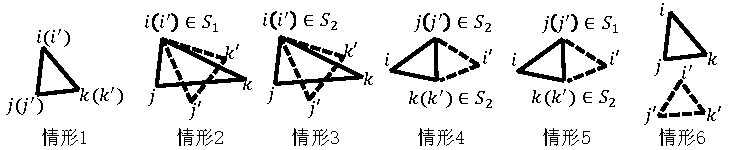
\includegraphics[width=\textwidth]{illustration_discrete_triangles.pdf}    
  \caption{关于两个三角形的重合情况讨论}\label{fig:illustration_triangles}
  \end{figure}
	\begin{enumerate}
		\item $\{i,j,k\} = \{i',j',k'\}$,则 $E[Y_{ijk}Y_{i'j'k'}] = pq^2$。
		在 $\E[T^2]$的求和式中共有 $n\binom{n}{2}$ 
     项。以下五种情形均需考虑$\E[T^2]$ 中出现的2倍的系数。
		\item 若 $\{i,j,k\}$ 和 $\{i',j',k'\}$ 只有
    一个共同的元素
    并且这个元素在 $ S_1$ 中, 则 $\E[Y_{ijk}Y_{i'j'k'}] = p^2q^4$。
		在 $\E[T^2]$的求和式中共有 $6n\binom{n}{4}$ 项 ($\binom{4}{2}=6$)。
		\item 若 $\{i,j,k\}$ 和 $\{i',j',k'\}$ 只有一个共同的元素
    并且这个元素 在 $ S_2$ 中,则
    $E[Y_{ijk}Y_{i'j'k'}] = p^2q^4$。在 $\E[T^2]$的求和式
		中共有 $12\binom{n}{2}\binom{n}{3}$ 项。
		\item 若 $\{i,j,k\}$ 和 $\{i',j',k'\}$ 恰有 两  个 共同的元素
    并且这两个元素均在 $S_2$ 中,
    则 $E[Y_{ijk}Y_{i'j'k'}] = pq^4$。
    在 $\E[T^2]$的求和式
		中共有  $2\binom{n}{2}\binom{n}{2}$ 项。
\item 若 $\{i,j,k\}$ 和 $\{i',j',k'\}$ 恰有两  个 共同的元素
且一个在 $S_1$ 中,另一个在 $S_2$ 中,则 $E[Y_{ijk}Y_{i'j'k'}] = p^2q^3$。
在 $\E[T^2]$的求和式
		中共有 $6n\binom{n}{3}$ 项。
\item  若 $\{i,j,k\}$ 和 $\{i',j',k'\}$ 没有共同的元素,
 则 $E[Y_{ijk}Y_{i'j'k'}] = p^2q^4$。
 在 $\E[T^2]$的求和式中共有 $12\binom{n}{2}\binom{n}{4}$ 
 项。
	\end{enumerate}
通过下面的求和式可以验证我们已经遍历了所有的情形:
% Mathematica Code:
% Simplify[n^2 (n-1)/2 + 12 Binomial[n,2] Binomial[n,3] + 6 n Binomial[n,4] + Binomial[n,4] Binomial[n,2]*12 + 6 n Binomial[n,3]+ 2 Binomial[n,2]^2]
\begin{equation}\label{eq:ver_nn2}
  n\binom{n}{2} + 6n\binom{n}{4} + 12\binom{n}{2} \binom{n}{3} + 2\binom{n}{2}^2 + 6n\binom{n}{3} + 12\binom{n}{2}\binom{n}{4} = \left(n\binom{n}{2}\right)^2  
\end{equation}
式\eqref{eq:ver_nn2}右端中出现的$n\binom{n}{2}$ 是$\E[T] $ 中求和式的项数。
\end{proof}
\begin{lemma}\label{lem:SBM_tr_counting_3}
	考虑 $\SSBM(3n, 3, p, q)$。它有3个社团,记为
  $S_1,S_2$ 和 $S_3$。
  计算满足如下条件的三角形的个数 $T$:
  这些三角形 有一个顶点在$S_1$中,有一个顶点在 $S_2$中,
  有一个顶点在 $S_3$ 中。
	则 $T$ 的方差为:
	\begin{equation*}\label{eq:SBM_tr_counting_three}
	\Var[T] = n^3 q^3  + 3n^3(n-1) q^4  + 3 n^3 (n-1)^2 q^5 - n^3(3n^2-3n+1)q^6
	\end{equation*}
\end{lemma}

\begin{proof}
	与引理 \ref{lem:SBM_tr_counting_cross} 的证明类似,
	$\E[T] = n^3 q^3$,对于$\E[T^2]$求和式中的项共如下4种情形:
	\begin{enumerate}
	\item 若 $\{i,j,k\} = \{i',j',k'\}$, 则 $E[Y_{ijk}Y_{i'j'k'}] = q^3$。
	$\E[T^2]$中 共有 $n^3$ 项。
	\item 若 $\{i,j,k\}$ 和 $\{i',j',k'\}$ 有一个共同的元素, 则 $E[Y_{ijk}Y_{i'j'k'}] = q^5$。
	$\E[T^2]$中 共有 $12n\binom{n}{2}^2$ 项。
	\item 若 $\{i,j,k\}$ 和 $\{i',j',k'\}$ 有两个共同的元素, 则 $E[Y_{ijk}Y_{i'j'k'}] = q^4$。
	$\E[T^2]$中 共有 $6\binom{n}{2}n^2$ 项。
	\item 若 $\{i,j,k\}$ 和 $\{i',j',k'\}$ 没有共同的元素, 则  $E[Y_{ijk}Y_{i'j'k'}] = q^6$。
	$\E[T^2]$中 共有 $8\binom{n}{2}^3$ 项。
\end{enumerate}	
通过下面的求和式可以验证我们已经遍历了所有的情形:
$$
6\binom{n}{2}n^2  + 8\binom{n}{2}^3 + 12n\binom{n}{2}^2 +  n^3 = n^6
$$
\end{proof}
\begin{lemma}\label{lem:sbmV}
 对于 $\SSBM(n, k, p, q)$,其中 $p=\frac{a\log n}{n}, q = \frac{b\log n}{n}$。
 三角形的数量为 $T$。
	则 $\frac{T}{(\log n)^3}$ 依概率收敛到 $\frac{1}{k^2}(\frac{a^3}{6} + \frac{k-1}{2}ab^2 + (k-1)(k-2)\frac{b^3}{6} )$。
\end{lemma}
\begin{proof}
 我们将 $T$ 分成三部分:
 第一部分是每个社团内部的三角形,记社团$i$里有$T_i$个三角形,则共有$k$个$T_i$的项。
 第二部分包括有一个点在第 $i$ 个社团内部,它所对的边在第$j$个社团里的那些三角形,记为 $T_{ij}$。
 共有 $k(k-1)$ 个 $T_{ij}$ 的项。第三部分包括三个顶点分别在$i,j,k$三个不同社团的三角形,共有
 $\binom{n}{3}$ 项。
	
	我们只需证明:
\begin{align}
	\frac{T_i}{\log ^3 n} &\xrightarrow{p} \frac{(a/k)^3}{6} \\
	\frac{T_{ij}}{\log^3 n}& \xrightarrow{p}\frac{1}{2}(a/k)(b/k)^2\\
	\frac{T_{ijk}}{\log^3 n} & \xrightarrow{p} (b/k)^3
	\end{align}
	
	$\frac{T_i}{\log ^3 n}$ 的收敛性可以直接从引理
 \ref{lem:ER_tr_counting} 中得到。这里,我们视$p=\frac{(a/k) (
    \log (n/k) + \log k)}{(n/k)}$,因为 $\log k$ 相比于其前一项量阶更小,
    可以忽略不计。
	对于 $T_{ij}$, 我们使用 
  引理 \ref{lem:SBM_tr_counting_cross}  的结果。
	在 式\eqref{eq:SBM_tr_counting_cross} 中
  我们用 $n/k$ 代替 $n$, 取 $p=a\frac{\log n}{n}$ 且 $q=b\frac{\log n}{n}$。
	$\Var[T_{ij}] \sim \frac{ab^2}{2k^3} \log^3 n$。
  因为 $\frac{T_{ij}}{\log^3 n}$ 的期望值是
  $(n/k)\binom{n/k}{2}pq^2/(\log^3 n)
	=\frac{n-1}{2n}\frac{ab^2}{k^3}$, 由切比雪夫不等式
  可得:
	\begin{align*}
	P \left( \left|\frac{T_{ij}}{\log^3 n} - \frac{n-1}{2n}\frac{ab^2}{k^3} \right| > \epsilon
  \right) &\leq \frac{\Var\left[T_{ij} / \log^3 n \right]}{\epsilon^2} \\
	& = \frac{1}{\epsilon^2}
	O \left( \frac{1}{\log^3 n} \right)
	\end{align*}
	
	因此, $\frac{T_{ij}}{\log^3 n} $ 依概率收敛到 $\frac{1}{2}(a/k)(b/k)^2$。
	
	为证明
  $\frac{T_{ijk}}{\log^3 n}\to (b/k)^3$,
  从 引理 \ref{lem:SBM_tr_counting_3} 中
  可得 $\Var[T_{ijk}] = O\left(\log^5 n\right)$:
	$$
	P \left( \left|\frac{T_{ijk}}{\log^3 n} -\frac{b^3}{k^3} \right| > \epsilon
  \right) \leq \frac{\Var \left[T_{ijk} / \log^3 n \right]}{\epsilon^2} = \frac{1}{\epsilon^2}
	O \left(\frac{1}{\log n} \right)
	$$
\end{proof}
\begin{proof}[定理 \ref{thm:ab12} 的证明]
	令 $e^*_1 = \frac{a+(k-1)b}{2k}$, $k^2 e^*_2 = \frac{a^3}{6} + \frac{k-1}{2}ab^2 + (k-1)(k-2)\frac{b^3}{6}$
	且 $e_1 = \frac{T_1}{n\log n}, e_2 = \frac{T_2}{\log^3 n}$。
	由 引理
  \ref{lem:ER_tr_counting}, $e_1 \to e^*_1$。
	由 引理 \ref{lem:sbmV}, 当 $n\to \infty$ 时,
  $e_2 \to e^*_2$。
	通过变量替换 $x=2ke_1 - (k-1)y$ 进行消元,
  我们可将
  方程组\eqref{eq:e_1}
  化简为如下的非线性方程:
\begin{equation}\label{eq:gy_y3}
g(y): = (k-1)(y^3 - 6 e_1 y^2 + 12 e_1^2 y) + 6 e_2 - 8 k e_1^3 = 0
\end{equation}

$g'(y) = 3(k-1)(y-2e_1)^2 \geq 0 $,
$g(y)$ 是$\mathbb{R}$上的增函数,
因此方程\eqref{eq:gy_y3} 最多有一个实根。
下面我们证明式\eqref{eq:gy_y3}有一个实根
在 区间 $(0, 2e_1)$ 内。
\begin{align*}
\lim_{n\to \infty}g(0) &=  6e^*_2 - 8k(e^*_1)^3  \\
&=-\frac{3}{k^2}(k-1)(k-2)ab^2-\frac{3(k-1)}{k^2}a^2b - \frac{k-1}{k^2} ((k-2)-(k-1)^2)b^3 < 0 \\
\lim_{n\to \infty}g(2e_1) &= 6e^*_2 - 8(e^*_1)^3 = \frac{(k-1)(a-b)^3}{k^3} > 0
% verified with sympy
\end{align*}

因此,由零值定理可得式\eqref{eq:gy_y3}有一个实根。由 $g(y)$的连续性,当$n\to \infty $ 时,该实根收敛到 $b$。
从而我们得到方程组\eqref{eq:e_1}有唯一解 $\hat{a},\hat{b}$,
且
$\hat{b} \to b$, $\hat{a} \to a$。
\end{proof}




\subsection{定理 \ref{thm:phase_transition} 的证明}
\label{sec:appendix_theorem_proof_phase_trans}

在开始定理 \ref{thm:phase_transition} 的技术证明之前,
我们需要介绍一些辅助的
符号。


注释 \ref{re:energy_diff} 中指出了
$X$改变一个状态前后的能量差表达式。
对于一般的情形,即改变
$|\cI|:=\Dist(\bar{\sigma}, X)$
个位置的状态后,
我们可以将能量差写成:
\begin{equation}\label{eq:Hgeneral}
H(\bar{\sigma}) - H(X)=
\left(1 + \gamma \frac{ \log n}{n} \right)[A_{\bar{\sigma}} - B_{\bar{\sigma}}] + \gamma\frac{ \log n}{n} N_{\bar{\sigma}}
\end{equation}
在上式中 我们使用
$A_{\bar{\sigma}}$ 或
$B_{\bar{\sigma}}$ 来表示
服从参数分别为 $\A$ 或 $\B$ 的二项分布的随机变量,并且
$N_{\bar{\sigma}}$ 是一个依赖于 $\bar{\sigma}$ 但与图结构无关的非随机的正整数。
引理 \ref{lem:minus}  给出了 $A_{\bar{\sigma}}, B_{\bar{\sigma}}$ 和 $N_{\bar{\sigma}}$
的表达式:

\begin{lemma}\label{lem:minus}
	对于 $\SSBM(n,k,p,q)$,
  我们假设 $\bar{\sigma}$ 
  在总共$|\cI|:=\Dist(\bar{\sigma}, X)$ 
  个坐标位置上不同于真值标签向量
  $X$。
	对于 $i\neq j$,令 $I_{ij} = \Big|\{r\in [n] \big| X_r = w^i, \sigma_r = w^j \}\Big|$
  且 $I_{ii} = 0$。
  我们进一步将行和$I_i$
  和列和$I'_i$分别表示为:
  \begin{align}
  I_i &= \frac{n}{k} -
  \Big|\{r\in [n] \big| X_r = w^i, \sigma_r=w^i \}\Big|
  =
  \sum_{j=0}^{k-1} I_{ij} \label{eq:I_i_horizontal} \\
  I'_i &=
  \Big|\{r\in [n] \big| X_r \neq w^i,
  \sigma_r=w^i \}\Big|
  =\sum_{j=0}^{k-1} I_{ji}\label{eq:I_prime_i_vertical}
  \end{align}
	则
\begin{align}
	N_{\bar{\sigma}} &= \frac{1}{2}\sum_{i=0}^{k-1} (I_i - I_i')^2 \label{eq:N_w} \\
	B_{\bar{\sigma}} & \sim \Binom(N_{B_{\bar{\sigma}}} , q),
  N_{B_{\bar{\sigma}}}=\frac{n}{k}|\cI| + \frac{1}{2}\sum_{i=0}^{k-1}  
  \left(-2 I'_i I_i  + I'^2_i - \sum_{j=0}^{k-1} I^2_{ji} \right)
  \label{eq:B_w}\\
	A_{\bar{\sigma}} &
  \sim \Binom(N_{A_{\bar{\sigma}}}, p),
  N_{A_{\bar{\sigma}}}=
  \frac{n}{k}|\cI| - \frac{1}{2}\sum_{i=0}^{k-1}
   \left(I^2_i + \sum_{j=0}^{k-1} I^2_{ij} \right)
  \label{eq:A_w}
	\end{align}
\end{lemma}
\begin{proof}
  由式\eqref{eq:isingma}、\eqref{eq:energy}可得
	\begin{align}
  \log P_{\sigma|G}(\sigma=\bar{\sigma})
  & = 
  \beta\left(1 + \frac{\gamma \log n}{n}\right) \sum_{\{i,j\} \in E(G)}  \delta(\bar{\sigma}_i, \bar{\sigma}_j)  
	\notag\\
  &\quad- \beta\frac{\gamma \log n}{n} \sum_{1\leq i<j \leq n} \delta(\bar{\sigma}_i, \bar{\sigma}_j) 
  - \log Z_G(\beta, \gamma) \notag\\
  & = 
  \beta\left(1 + \frac{\gamma \log n}{n}\right) \sum_{\bar{\sigma}_i = \bar{\sigma}_j} Z_{ij}
	- \beta\frac{\gamma \log n}{n}
  \sum_{\bar{\sigma}_i = \bar{\sigma}_j} 1 
  - \log Z_G(\beta, \gamma)
  \label{eq:log_P_sigma_G_bar_sigma}
  \end{align}
	其中 $Z_{ij}$ 服从伯努利分布,
  $P(Z_{ij}=1)$ 表示节点$i$与节点$j$之间有边相连的概率。
	对于 $\sigma = X$, 我们有
	\begin{align}
	\sum_{X_i = X_j} Z_{ij} &
  = \sum_{X_i = X_j, \bar{\sigma}_i = \bar{\sigma}_j}
  Z_{ij} + \sum_{X_i = X_j, \bar{\sigma}_i \neq \bar{\sigma}_j}
  Z_{ij}
  \label{eq:split_zij_tmp_X_ij}\\
	\sum_{X_i = X_j} 1 &= \frac{1}{2} \sum_{i=0}^{k-1} \frac{n}{k} 
  \left( \frac{n}{k} - 1 
  \right)\label{eq:split_one_tmp_X_ij}
	\end{align}
	对于 $\sigma = \bar{\sigma}$,我们有
	\begin{align}
	\sum_{\bar{\sigma}_i = \bar{\sigma}_j} Z_{ij} &= \sum_{X_i = X_j, \bar{\sigma}_i = \bar{\sigma}_j} Z_{ij} + \sum_{X_i \neq X_j, \bar{\sigma}_i = \bar{\sigma}_j} Z_{ij} 
  \label{eq:split_zij_tmp_sigma_ij}\\
	\sum_{\bar{\sigma}_i = \bar{\sigma}_j} 1 &= \frac{1}{2} \sum_{i=0}^{k-1} 
  \left(I'_i + \frac{n}{k} - I_i \right)
  \left( I'_i + \frac{n}{k} - I_i - 1 \right)
  \label{eq:split_one_tmp_sigma_ij}
	\end{align}
  其中,式 \eqref{eq:split_one_tmp_sigma_ij} 是根据式
  \eqref{eq:I_i_horizontal}和 \eqref{eq:I_prime_i_vertical}
  而来。
	注意到
  $
  \Big|\{r\in [n] \big| X_r = w^i, \sigma_r=w^i \}\Big|
  =\frac{n}{k} - I_i$和
	$|\{r\in [n] | X_r \neq \omega^i, \sigma_r = \omega^i \}| = I'_i$,
	我们因此有  
  \begin{equation}\label{eq:number_of_sigma_r_equal_omega_i}
    |\{r\in [n] | \sigma_r = \omega^i \}|
    = I'_i + \frac{n}{k} - I_i
  \end{equation}
  类比式\eqref{eq:split_one_tmp_X_ij}从而得到
  式\eqref{eq:split_one_tmp_sigma_ij}。

  由式\eqref{eq:Pratio} 我们得到
  \begin{equation}
    \frac{P_{\sigma |G } (\sigma = \bar{\sigma})}
    {P_{\sigma |G } (\sigma = X)}
    = \exp(-\beta(H(\bar{\sigma})
    - H(X)))
  \end{equation}
  结合式\eqref{eq:log_P_sigma_G_bar_sigma}
  可得
  \begin{equation}\label{eq:Hgeneral_tmp_derived}
    H(\bar{\sigma}) - H(X)=
    -\left(1 + \gamma \frac{ \log n}{n}
    \right)
    \left[
      \sum_{\bar{\sigma}_i = \bar{\sigma}_j}Z_{ij} - \sum_{X_i = X_j}Z_{ij}
      \right]
    + \gamma\frac{ \log n}{n}
    \left[\sum_{\bar{\sigma}_i = \bar{\sigma}_j}1 - \sum_{X_i = X_j}1
    \right]
    \end{equation}
  将式\eqref{eq:Hgeneral_tmp_derived} 与式\eqref{eq:Hgeneral}
  对比可得:
  \begin{align}
    B_{\bar{\sigma}} - A_{\bar{\sigma}} &=
    \sum_{\bar{\sigma}_i = \bar{\sigma}_j}Z_{ij}
    - \sum_{X_i = X_j}Z_{ij}
    \label{eq:B_bar_A_bar_lem_minus}\\
    N_{\bar{\sigma}} &=
    \sum_{\bar{\sigma}_i = \bar{\sigma}_j} 1  -\sum_{X_i = X_j} 1
    \label{eq:N_bar_sigma_lem_minus}
  \end{align}
  由式\eqref{eq:split_one_tmp_X_ij}、
  \eqref{eq:split_one_tmp_sigma_ij}、 
  \eqref{eq:N_bar_sigma_lem_minus} 可得
  $N_{\bar{\sigma}} = \sum_{\bar{\sigma}_i = \bar{\sigma}_j} 1  -\sum_{X_i = X_j} 1 = \frac{1}{2}\sum_{i=0}^{k-1} (I_i - I_i')^2 $,
  即式 \eqref{eq:N_w}。
	另一方面,由式\eqref{eq:B_bar_A_bar_lem_minus}、
  \eqref{eq:split_zij_tmp_X_ij}、 
  \eqref{eq:split_zij_tmp_sigma_ij}
  可得 $B_{\bar{\sigma}} - A_{\bar{\sigma}} = \sum_{X_i \neq X_j, \bar{\sigma}_i = \bar{\sigma}_j} Z_{ij} - \sum_{X_i = X_j, \bar{\sigma}_i \neq \bar{\sigma}_j} Z_{ij}$。
	对于在求和式 $\sum_{X_i \neq X_j, \bar{\sigma}_i = \bar{\sigma}_j} Z_{ij}$
  中出现的 $Z_{ij}$, $Z_{ij} \sim \Bern(q)$
  并且我们有
  \begin{align}
  \sum_{X_i \neq X_j, \bar{\sigma}_i = \bar{\sigma}_j} 1 
  &= \sum_{i=0}^{k-1}
  \left[
    \left(\frac{n}{k} - I_i \right)
    I_i' + \frac{1}{2} \sum_{j=0}^{k-1} I_{ji}(I'_i - I_{ji}) 
  \right] 
  \label{eq:x_i_neq_x_j_bar_sigma_i_eq_bar_sigma_j_0}\\
	&=\frac{n}{k}|\cI| + \frac{1}{2}\sum_{i=0}^{k-1}  
  \left(-2 I'_i I_i  + I'^2_i - \sum_{j=0}^{k-1} I^2_{ji}\right) 
  \label{eq:x_i_neq_x_j_bar_sigma_i_eq_bar_sigma_j_1}
  \end{align}
  在式\eqref{eq:x_i_neq_x_j_bar_sigma_i_eq_bar_sigma_j_0}
  最外层的求和中,首先遍历的是$X_i=1, \omega, \dots, \omega^{k-1}$。  
  而式\eqref{eq:split_one_tmp_sigma_ij}
  利用了
  $|\cI| = \sum_{i=0}^{k-1} I'_i$。
  类似的,
  对于在求和式 $\sum_{X_i = X_j, \bar{\sigma}_i \neq \bar{\sigma}_j} Z_{ij}$
  中出现的 $Z_{ij}$, $Z_{ij} \sim \Bern(p)$。
	$\sum_{X_i = X_j, \bar{\sigma}_i \neq \bar{\sigma}_j} 1
	= \sum_{i=0}^{k-1}[(\frac{n}{k} - I_i) I_i + \frac{1}{2} \sum_{j=0}^{k-1} I_{ij}(I_i - I_{ij}) ] 
	= \frac{n}{k}|\cI| - \frac{1}{2}\sum_{i=0}^{k-1}  (I^2_i + \sum_{j=0}^{k-1} I^2_{ij})$。
  从而式\eqref{eq:B_w}、\eqref{eq:A_w} 得证。
\end{proof}

从上面可以看到引理 \ref{lem:minus} 的证明并没有很多技巧性,主要涉及一些计数
的技巧。
当 $|\cI|$ 相比  $n$ 很小时
我们有如下的引理, 该引理是 文献\inlinecite{ye2020exact} 中 陈述 6 的拓展。 

\begin{lemma}
  \label{lem:enhanced_fb}
	对于 $t\in [\frac{1}{k}(b-a), 0], 0<\delta <1$
	和 $ |\cI| \le n/\log^{\delta} n$,我们有
\begin{equation} \label{eq:upmpt}
	P_G(B_{\bar{\sigma}}-A_{\bar{\sigma}}\ge t |\cI| \log n) 
	\le  \exp\Big(|\cI|\log n\cdot
	\left(
    f_{\beta}(t) - \beta t -1	+ O((\log n)^{-\delta}) \right)\Big)
	\end{equation}
	其中 $f_{\beta}(t) := \min_{s\geq 0} (g(s) - st) + \beta t \leq \tilde{g}(\beta) $。
  函数$g(\beta), \tilde{g}(\beta)$
  的定义分别参见
  式\eqref{eq:g_beta_main_article}
  和
  \eqref{eq:g_tilde_beta_main_article} 。
\end{lemma}

在引理 \ref{lem:enhanced_fb}  中,
取
$|\cI|=1, N_{\bar{\sigma}}=0$,
此时$A_{\bar{\sigma}} \sim \Binom(\frac{n}{k}, \A),
B_{\bar{\sigma}} \sim \Binom(\frac{n}{k}, \B)$,
即得到 式\eqref{eq:introduction_g_a_b_eps}。

\begin{proof}[引理 \ref{lem:enhanced_fb} 的证明]
  由函数$f_{\beta}(t)$的定义,
  式\eqref{eq:upmpt}中
  $f_{\beta}(t) - \beta t$ 与$\beta$无关而只与
  $t$有关。
	由定义可知,
  $A_{\bar{\sigma}}\sim \Binom(N_{A_{\bar{\sigma}}},\frac{a\log n}{n})$
  且
	$B_{\bar{\sigma}}\sim\Binom(N_{B_{\bar{\sigma}}},\frac{b\log n}{n})$,
  并且二者彼此独立。
  由 ( \ref{eq:N_w}-\ref{eq:A_w} )可知,$N_{B_{\bar{\sigma}}} - N_{A_{\bar{\sigma}}}
  = N_{\bar{\sigma}}$。
  对于$s>0$,
  $B_{\bar{\sigma}}-A_{\bar{\sigma}}$ 的矩生成函数可以展开成
	\begin{align}
	 \mathbb{E}[e^{s(B_{\bar{\sigma}}-A_{\bar{\sigma}})}] 
	& =\Big(1-\frac{b\log n}{n}+\frac{b\log n}{n} e^s \Big)^{N_{B_{\bar{\sigma}}}}
	\Big(1-\frac{a\log n}{n}+\frac{a\log n}{n} e^{-s} \Big)^{N_{A_{\bar{\sigma}}}}  \notag\\
	& = \exp\left(\frac{\log n}{n}\left(N_{B_{\bar{\sigma}}}
  (be^s - b) + N_{A_{\bar{\sigma}}}(ae^{-s}-a) + N_{B_{\bar{\sigma}}}
  O \left(\frac{\log n}{n} \right) \right) \right)
  \label{eq:exp_s_B_A_sigma}
	\end{align}
	由\eqref{eq:B_w}
  和\eqref{eq:A_w},并
  注意到$k$是个常数,
  当
  $|\cI| \le n/\log^{\delta}(n)$ 时
	我们能估计
  $N_{B_{\bar{\sigma}}}$和$N_{A_{\bar{\sigma}}}$
  的阶数。它们分别是
  $N_{A_{\bar{\sigma}}} = \frac{n}{k}|\cI| + O(|\cI|^2)$,
	 $N_{B_{\bar{\sigma}}} = \frac{n}{k}|\cI| + O(|\cI|^2)$。
   由此得
	\begin{align*}
	\mathbb{E}[e^{s(B_{\bar{\sigma}}-A_{\bar{\sigma}})}]
  & \le
	\exp\left(\frac{\log n}{n}\Big( 
    \left(\frac{n}{k}|\cI| + O\left(|\cI|^2\right)\right)
    (be^s - b) 
    \right.\\
  & \left. \quad 
  + \left(\frac{n}{k} |\cI| + O(|\cI|^2)\right)(ae^{-s}-a) + \frac{n}{k}|\cI|O\left(\frac{\log n}{n} \right) \Big)\right)\\
	&=
   \exp\left(\frac{|\cI| \log n}{k}
   \left(a e^{-s}+b e^s-a-b +
	O \left(\log^{-\delta}(n) \right) \right) \right)
	\end{align*}
	最后一个等式来自于
  $ |\cI| \le n/\log^{\delta}(n)$这个假设。
	由切尔诺夫不等式(参见 \eqref{eq:chernoff_bound}),
  对于 $s>0$,我们有
	\begin{align*} 
	P_G(B_{\bar{\sigma}}-A_{\bar{\sigma}}\ge t |\cI| \log n)
  & \le
	\frac{\mathbb{E}[e^{s(B_{\bar{\sigma}}-A_{\bar{\sigma}})}]}{e^{st |\cI|  \log n}}  \\
  &\le \exp\Big(\frac{|\cI|\log n}{k} \big(a e^{-s}+b e^s -kst -a-b
	+ O(\log^{-\delta}(n)) \big)\Big) 
	\end{align*}
	上式右端对$s\geq 0$取最小值即有
  \eqref{eq:upmpt}。  
	\end{proof}

  对应于定理 \ref{thm:phase_transition}  的三种情况,我们还需要使用若干个非平凡的引理来辅助证明。

  \begin{lemma}\label{lem:sigmaX}
    令 $\gamma > b$, 且 $\bar{\sigma}$ 满足 $\Dist(\bar{\sigma}, X) \geq \frac{n}{\sqrt{\log n}}$
    和 $\Phi(\bar{\sigma}, X)=1$
    (参见\eqref{eq:D_sigma_sigma_prime})
    两个条件。
    则事件
    $P_{\sigma | G}(\sigma = \bar{\sigma} ) > \exp(-Cn) P_{\sigma | G}(\sigma = X)$
    发生的概率小于 $\exp(-\tau(\beta, \gamma) n \sqrt{\log  n} )$,
    其中 $C$ 是任意事先给定的常数而 
    $\tau(\beta, \gamma)$
   是某个依赖于$\beta$ 和 $\gamma$的取值为正值的函数。
  \end{lemma}
  \begin{proof}
    我们把 事件 $P_{\sigma | G}(\sigma = \bar{\sigma} ) > \exp(-Cn) P_{\sigma | G}(\sigma = X)$
    记为 $\widetilde{D}(\bar{\sigma}, C)$。
    由式 \eqref{eq:Hgeneral}, $\widetilde{D}(\bar{\sigma}, C)$
    等价于:
  \begin{equation}\label{eq:BwA}
    \left(1 + \frac{\gamma \log n}{n} \right)
    [B_{\bar{\sigma}} - A_{\bar{\sigma}}] >  \frac{\gamma \log n}{n} N_{\bar{\sigma}}  - \frac{C}{\beta} n
    \end{equation}  
    
    我们声称$\bar{\sigma}$  必须满足以下两个条件中的至少一个。
    \begin{enumerate}
      \item $\exists i\neq j$ 使得 $\frac{1}{k(k-1)}\frac{n}{\sqrt{\log n}} \leq I_{ij} \leq \frac{n}{k} - \frac{1}{k(k-1)}\frac{n}{\sqrt{\log n}}$
      \item $\exists i \neq j$ 使得 $I_{ij} > \frac{n}{k} - \frac{1}{k(k-1)}\frac{n}{\sqrt{\log n}}$ 且 $I_{ji} < \frac{1}{k(k-1)}\frac{n}{\sqrt{\log n}}$
    \end{enumerate}
    $I_{ij}$的定义参见引理
    \ref{lem:minus}。
    如果上面两个条件均不成立,则由条件1,对 $0 \leq i,j\leq k-1$,
    我们有
    $I_{ij} < \frac{1}{k(k-1)}\frac{n}{\sqrt{\log n}}$
    或者 $I_{ij} > \frac{n}{k} - \frac{1}{k(k-1)}\frac{n}{\sqrt{\log n}}$。
    
    因为 $\sum_{i,j} I_{ij} = |\cI| \geq \frac{n}{\sqrt{\log n}}$,
    存在 $i,j$ 使得
    $I_{ij} > \frac{n}{k} - \frac{1}{k(k-1)}\frac{n}{\sqrt{\log n}}$。
    对于这一对确定的 $i,j$,不妨先假设 $I_{ji} > \frac{n}{k} - \frac{1}{k(k-1)}\frac{n}{\sqrt{\log n}}$,
    下面我们将推出矛盾说明该假设不成立。
    取 $X'$ 为在$X$ 的基础上交换$w^i$ 和 $w^j$ 位置后的向量,
    然后我们考虑
  \begin{align}
     \Dist(\bar{\sigma}, X')  - \Dist(\bar{\sigma}, X)
     &= |\{ r \in [n]|X_r=w^i, \bar{\sigma}_r \neq w^j \}| 
     + |\{ r \in [n]|X_r=w^j, \bar{\sigma}_r \neq w^i \}|\notag\\ 
    &-|\{ r \in [n]|X_r=w^i, \bar{\sigma}_r \neq w^i \}| 
    - |\{ r \in [n]|X_r=w^j, \bar{\sigma}_r \neq w^j \}| \notag\\
    & = \frac{n}{k} - I_{ij} +  \frac{n}{k} - I_{ji} - I_i - I_j\label{eq:distsmall} \\
    & < \frac{2}{k(k-1)}\frac{n}{\sqrt{\log n}} - I_i - I_j < 0\notag
    \end{align}
    这和 $\bar{\sigma}$ 离 $X$ 最近的条件矛盾。
    因此
    $I_{ji} > \frac{n}{k} - \frac{1}{k(k-1)}\frac{n}{\sqrt{\log n}}$
    不成立,由条件1
    则有  $I_{ji} < \frac{1}{k(k-1)}\frac{n}{\sqrt{\log n}}$。
    但这样一来 $(i, j)$ 二元组满足 条件 2,
    又与 $\bar{\sigma}$ 不满足如上两个条件的假设相矛盾。
    
    在条件1的假设下,我们能获得 $N_{A_{\bar{\sigma}}}$的一个下界。
    为方便估计该下界,我们首先改写式\eqref{eq:A_w}。
    对于 $i\neq j$,令 $I'_{ij} = I_{ij}$,
    而 $I'_{ii} = \frac{n}{k} - I_i$。
    则我们有:
    \begin{align*}
    N_{A_{\bar{\sigma}}} &=
    \frac{n}{k}|\cI| - \frac{1}{2}\sum_{i=0}^{k-1}
    \left(I^2_i + \sum_{j=0}^{k-1} I^2_{ij} \right) \\
    &=
    \frac{n}{k}|\cI| - \frac{1}{2}\sum_{i=0}^{k-1}
    \left(\left(\frac{n^2}{k^2} - 2\frac{n}{k} I'_{ii} \right) +
    \sum_{j=0}^{k-1} I'^2_{ij} \right) \\
    &=
    \frac{n}{k}|\cI| - \frac{1}{2}\sum_{i=0}^{k-1}
    \left(\left(\frac{n^2}{k^2} - 2\frac{n}{k} \left(\frac{n}{k} - I_i\right)\right)\right)
    - \frac{1}{2}\sum_{i=0}^{k-1}\sum_{j=0}^{k-1} I'^2_{ij} \\
    &= \frac{n^2}{2k} - \frac{1}{2}
    \sum_{i=0}^{k-1} \sum_{j=0}^{k-1} I'^2_{ij}
   \end{align*}
    
    在求和式中 $\sum_{i=0}^{k-1} \sum_{j=0}^{k-1} I'^2_{ij}$
    的每一项 $\sum_{j=0}^{k-1} I'^2_{ij}$
    均满足 $\sum_{j=0}^{k-1}
    I'_{ij} = \frac{n}{k}$,当某个$I'_{ii}$取$\frac{n}{k}$
    而其余的项为零时$\sum_{j=0}^{k-1} I'^2_{ij}$
    最大。但由于条件1成立,有某一行不能取
    这种极端值,所以 $\sum_{i=0}^{k-1} \sum_{j=0}^{k-1} I'^2_{ij}$中
    共有 $(k-1)$行求和得$ (k-1)\frac{n^2}{k^2}$
    而其中一行则必须保留$I'_{ij}, I'_{ii}$ 这两个非零项。
    因此
    $\sum_{i=0}^{k-1} \sum_{j=0}^{k-1} I'^2_{ij}
    \leq (k-1)\frac{n^2}{k^2} + (\frac{n}{k} - I_{ij})^2 + I^2_{ij}$,
    而这里的
    $I_{ij}$ 满足条件1。
    进一步的, $\sum_{i=0}^{k-1} \sum_{j=0}^{k-1} I'^2_{ij} \leq (k-1)\frac{n^2}{k^2} + 
    \left(\frac{1}{k(k-1)}\frac{n}{\sqrt{\log n}} \right)^2
    + \left(\frac{n}{k} - \frac{1}{k(k-1)}\frac{n}{\sqrt{\log n}} \right)^2 
    = \frac{n^2}{k} - \frac{2n^2}{k^2 (k-1)\sqrt{\log n}}(1+o(1))$。
    从而我们得到
  \begin{equation}\label{eq:Asigma}
    A_{\bar{\sigma}} \geq \frac{n^2}{k^2 (k-1)\sqrt{\log n}}(1+o(1))
    \end{equation}
    
    
    在条件2的假设下, 我们能得到
    $N_{\bar{\sigma}}$的一个下界。
    因为
    $\Dist(\bar{\sigma}, X') - \Dist(\bar{\sigma}, X) \geq 0$,
     由式 \eqref{eq:distsmall}  我们有
    $I_{ij} + I_{ji} + I_{i} + I_j \leq \frac{2n}{k} $。
    又因为 $I_i \geq I_{ij} > \frac{n}{k} - \frac{1}{k(k-1)}\frac{n}{\sqrt{\log n}}$,
    从而$I_j $ 满足
    $I_j \leq \frac{2}{k(k-1)}\frac{n}{\sqrt{\log n} }$。
    进一步有 $I'_j - I_j \geq I_{ij} - I_j \geq  \frac{n}{k} - \frac{3}{k(k-1)}\frac{n}{\sqrt{\log n} }$。
    由 式\eqref{eq:N_w}有
     $N_{\bar{\sigma}} \geq \frac{1}{2}
     \left(\frac{n}{k} - \frac{3}{k(k-1)}\frac{n}{\sqrt{\log n}} \right)^2 
     = \frac{n^2}{2k^2}(1+o(1))$。
    
    下面我们用
     切尔诺夫不等式给出式\eqref{eq:BwA}描述的事件发生概率的上界。
     在分析中我们可以省略不等号左边的 $\frac{\gamma \log n}{n}$ 一项
     ,因为其远小于$1$。
    令 $Z \sim \Bern\left(\A\right), Z' \sim \Bern\left(\B\right)$,则:
    \begin{align*}
    P_G(\widetilde{D}(\bar{\sigma}, C))
    &\leq (\mathbb{E}[\exp(sZ')])^{N_{B_{\bar{\sigma}}}}
    (\mathbb{E}[\exp(-sZ)])^{N_{A_{\bar{\sigma}}}}\cdot 
    \exp\left(
      -s\left(
        \frac{\gamma \log n}{n} N_{\bar{\sigma}}  - \frac{C}{\beta}n
      \right)
      \right) \\
    & \leq \exp\left(N_{B_{\bar{\sigma}}}
    \frac{b\log n}{n}(e^s -1) + 
    N_{A_{\bar{\sigma}}}\frac{a\log n}{n} \left(e^{-s} - 1 \right)\right. \\
    &\quad \left. - s \left(\frac{\gamma \log n}{n} N_{\bar{\sigma}} 
    - \frac{C}{\beta}n \right)
    \right) 
    \end{align*}
    
    使用 $N_{B_{\bar{\sigma}}} = N_{\bar{\sigma}} + N_{A_{\bar{\sigma}}}$
    我们可以进一步简化上式中的指数项为:
    $$
    \frac{\log n}{n} [N_{A_{\bar{\sigma}}}(b(e^s -1)+ a(e^{-s} - 1)) +
    N_{\bar{\sigma}} (b(e^s - 1)-\gamma s)]  + s \frac{C}{\beta}n
    $$
    
    下面我们考察 函数 $g_1(s) = b(e^s -1)+ a(e^{-s} - 1)$
    和 $g_2(s) = b(e^s - 1)-\gamma s$。
    两个函数 在 $s=0$ 处取值为零
    并且 $g_1'(s) = (be^s - ae^{-s}), g_2'(s) = be^s -\gamma$。
    因此, $g_1'(0) = b-a<0, g_2'(0) = b - \gamma < 0$。
    我们可以选择 $s^*>0$,使得 $g_1(s^*) < 0,g_2(s^*) < 0$。
    为了补偿 $sCn/\beta$ 这一项的影响,我们只需要确保
    $\frac{\log n}{n} \min\{N_{A_{\bar{\sigma}}}, N_{\bar{\sigma}}\}$ 的阶数大于$n$。
    由于   $N_{A_{\bar{\sigma}}}\geq \frac{n^2}{k^2 (k-1)\sqrt{\log n}}(1+o(1))$ 或 $N_{\bar{\sigma}} \geq \frac{n^2}{2k^2}(1+o(1))$
    有一个成立,
    这一要求得到了满足。
  \end{proof}

\begin{lemma}\label{prop:small}
  若 $\gamma>b$, $\beta>\beta^\ast$,
  对于 $1\leq r \leq \frac{n}{\sqrt{\log n}}$
  和 $\forall \epsilon > 0$,
  存在集合 $\cG^{(r)}$ 使得:
\begin{equation}\label{eq:Gr}
  P_G(\cG^{(r)}_n) \ge 1 - n^{r(\tilde{g}(\beta)/2 + \epsilon)}
  \end{equation}
  并且对于任意 $G\in\cG^{(r)}_n$,有
\begin{equation}\label{eq:psigmaX}
  \frac{P_{\sigma|G}(\Dist(\sigma, X)=r | \Phi(\sigma, X)=1)}
  {P_{\sigma|G}(\sigma=X | \Phi(\sigma, X)=1)} <
  n^{r \tilde{g}(\beta) /2}
  \end{equation}
  
  对于 $r> \frac{n}{\sqrt{\log n}}$, 存在集合 $\cG^{(r)}$, 使得:
\begin{equation}\label{eq:Gr1}
  P(G\in\cG^{(r)}_n) \ge 1 - e^{-n}
  \end{equation}
  并且对于任意 $G\in\cG^{(r)}_n$,有
\begin{equation}\label{eq:psigmaX1}
  \frac{P_{\sigma|G}(\Dist(\sigma, X)=r | \Phi(\sigma, X)=1)}
  {P_{\sigma|G}(\sigma=X | \Phi(\sigma, X)=1)} <
  e^{-n}
  \end{equation}
\end{lemma}
\begin{proof}
  我们分两种情况讨论: $r\leq \frac{n}{\sqrt{\log n}}$
  和 $r > \frac{n}{\sqrt{\log n}}$。
  
  当 $r\leq \frac{n}{\sqrt{\log n}}$ 时,
  通过使用 关于 $\Dist$
  的三角不等式,
  我们可以证明 
  $\Dist(\sigma, X) = r$ 蕴含
  $\Phi(\sigma, X)=1$。
   对于 $f \in S_k \backslash \{ \textrm{id} \}$,
   其中
   $\textrm{id}$ 是恒等映射,
   我们有:
  $$
  \frac{2n}{k} \leq \Dist(f(X), X) \leq \Dist(\sigma, f(X)) + \Dist(\sigma, X)
  $$
  
  因此,
  $\Dist(\sigma, f(X)) \geq \frac{2n}{k} - \frac{n}{\sqrt{\log n}} \geq \Dist(\sigma, X)$。
  从而我们得到
  式\eqref{eq:psigmaX}  等价于:
  \begin{equation}\label{eq:psigmaX2}
  \frac{P_{\sigma|G}(\Dist(\sigma, X)=r)}
  {P_{\sigma|G}(\sigma=X)} <
  n^{r \tilde{g}(\beta) /2}
  \end{equation}
  
  上式左边可以写为:
  \begin{align*}
  \frac{P_{\sigma|G}(\Dist(\sigma, X)=r)}
  {P_{\sigma|G}(\sigma=X)}  &= \sum_{\Dist(\bar{\sigma}, X)=r}\exp(-\beta(H(\bar{\sigma})-H(X)))\\
  \textrm{ 由 \eqref{eq:Hgeneral} } &\leq \sum_{\Dist(\bar{\sigma}, X)=r}\exp(\beta_n(B_{\bar{\sigma}}-A_{\bar{\sigma}}))
  \end{align*}
  其中 
  \begin{equation}\label{eq:beta_n_def}
  \beta_n = \beta \left(1+\gamma\frac{\log n}{n} \right)
  \end{equation}
  
  定义
  $\Xi_n(r): = \sum_{\Dist(\bar{\sigma}, X)=r}\exp(\beta_n(B_{\bar{\sigma}}-A_{\bar{\sigma}}))$,
  我们只需证明:
  \begin{equation}
  P_{G}(\Xi_n(r) \geq n^{r \tilde{g}(\beta) /2}) \leq  n^{r (\tilde{g}(\beta) /2 + \epsilon)}
  \end{equation}
  
  定义 事件 $\Lambda_n(G,r):=\{B_{\bar{\sigma}} -A_{\bar{\sigma}} < 0, \forall \bar{\sigma}\, \Dist(\bar{\sigma}, X)=r\}$,
  然后我们采用下面的方式进行处理:
  \begin{align*}
  P_{G}(\Xi_n(r) \geq n^{r \tilde{g}(\beta) /2}) \leq
  P_G(\Lambda_n(G,r)^c)
  + P_G\left(
    \Xi_n(r) \geq n^{r \tilde{g}(\beta) /2} |\Lambda_n(G,r) 
    \right)
  \end{align*}
  
  对于第一项, 因为
  $|\{ \bar{\sigma} | \Dist(\bar{\sigma}, X) = r \}| \leq (k-1)^r n^r$,
  由 引理 \ref{lem:enhanced_fb}  可得
  $P_G(\Lambda_n(G,r)^c) \leq (k-1)^r n^{rg(\bar{\beta})} \leq n^{r (\tilde{g}(\beta) /2 + \epsilon/2)}$。

  对于第二项,我们使用马尔可夫不等式:
  \begin{align*}
  P_G\left(\Xi_n(r) \geq n^{r \tilde{g}(\beta) /2} |\Lambda_n(G,r) \right)
  \leq \mathbb{E}[\Xi_n(r)|\Lambda_n(G,r)]n^{-r \tilde{g}(\beta) /2} 
  \end{align*}
  
  而上式中的条件期望可以做如下估计:
  \begin{align*}
  \mathbb{E}[\Xi_n(r)|\Lambda_n(G,r)]&=
  \sum_{\Dist(\bar{\sigma}, X) = r}\sum_{tr\log n = -\infty }^{-1} 
   P_G(B_{\bar{\sigma}} -A_{\bar{\sigma}}=tr\log n)\exp(\beta_n tr \log n) \\
  & \leq (k-1)^r n^{r+r\beta_n(b-a)/k} \\
  &\quad +
  \sum_{\Dist(\bar{\sigma}, X) = r}\sum_{tr\log n = r\frac{b-a}{k}\log n }^{-1} 
   P_G(B_{\bar{\sigma}} -A_{\bar{\sigma}}=tr\log n)\exp(\beta_n tr \log n)
  \end{align*}
  $1+\beta_n(b-a)/k = f_{\beta_n}(\frac{b-a}{k}) < \tilde{g}(\beta_n)$,
  因此,
  $(k-1)^r n^{r+r\beta_n (b-a)/k}n^{-r \tilde{g}(\beta) /2} \leq$
   $n^{r (\tilde{g}(\beta) /2 + \epsilon/2)} $。
  使用 引理 \ref{lem:enhanced_fb}, 我们有:
  \begin{align*}
  P_G(B_{\bar{\sigma}} -A_{\bar{\sigma}}=tr\log n)\exp(\beta_n rt \log n) \leq 
  n^{r(f_{\beta_n}(t)-1 + O(\frac{1}{\sqrt{\log n}}))}
  \end{align*}
  
  因为 $\beta_n \to \beta$, $\forall \epsilon$,
  当 $n$ 充分大时
  我们有 $\tilde{g}(\beta_n) \leq \tilde{g}(\beta) + \epsilon /2$。
  因此,
  \begin{align*}
  &n^{-r \tilde{g}(\beta) /2}\sum_{\Dist(\bar{\sigma}, X) = r}\sum_{\substack{tr\log n = \\ r(b-a)/k\log n} }^{-1}
  P_G(B_{\bar{\sigma}} -A_{\bar{\sigma}}=t\log n)\exp(\beta_n rt \log n) \\
  & \leq  \frac{(k-1)^r r(b-a)}{k} ( \log n )
  n^{r(\tilde{g}(\beta_n) - \tilde{g}(\beta)/2)}\\
  & \leq  n^{r(\tilde{g}(\beta)/2 + \epsilon/2)}  (k-1)^r O(\log n)
  \end{align*}
  
  结合上式, 我们可以得到:
  \begin{align*}
  P_{G}(\Xi_n(r) \geq n^{r \tilde{g}(\beta) /2}) &\leq  n^{r(\tilde{g}(\beta)/2 + \epsilon/2)}  (k-1)^r O(\log n)\\
  &\leq n^{r(\tilde{g}(\beta)/2 + \epsilon)}
  \end{align*}
  
  当 $r>\frac{n}{\sqrt{\log n}}$时,
  由引理 \ref{lem:sigmaX},
  我们选取充分大的常数  $C>1$
  使得 $k^n\exp(-Cn) < e^{-n}$:
  \begin{align*}
  &\frac{P_{\sigma|G}(\Dist(\sigma, X)=r | \Phi(\sigma, X)=1)}
  {P_{\sigma|G}(\sigma=X | \Phi(\sigma, X)=1)} = 
  \sum_{\substack{\Phi(\bar{\sigma}, X)=1 \\ 
  \Dist(\bar{\sigma}, X)=r}} \frac{P_{\sigma | G}(\sigma = \bar{\sigma}) }{P_{\sigma | X}(\sigma = X)} > \exp(-n)\\
  &\Rightarrow \exists \bar{\sigma},
  \frac{P_{\sigma | G}(\sigma = \bar{\sigma}) }{P_{\sigma | X}(\sigma = X)} > k^{-n}\exp(-n)
  \Rightarrow \exists \bar{\sigma},
  \frac{P_{\sigma | G}(\sigma = \bar{\sigma}) }{P_{\sigma | X}(\sigma = X)} > \exp(-Cn)\\
  \end{align*}
  最后一个事件发生的概率小于 $k^ne^{-\tau(\beta, \gamma) n\sqrt{\log n}}<e^{-n}$。
  因此,    式\eqref{eq:psigmaX1}成立。
  \end{proof}

  如果 $\gamma > b$ 且 $\beta < \beta^*$,则我们有如下的引理:
 \begin{lemma}\label{lem:7}
	若 $\gamma > b$ 且 $\beta < \beta^*$,
  则存在集合 $\cG^{(1)}_n$ 使得
	$P_G(\cG^{(1)}_n) \geq 1-n^{g(\bar{\beta})}$
	并且:
 \begin{align}
	\mathbb{E}\left[
    \sum_{r=1}^n \exp(\beta_n (A_r^s - A_r^0)) | G \in \   cG^{(1)}_n\right] &= (1+o(1))n^{g(\beta_n)} \\
	\Var \left[
    \sum_{r=1}^n \exp(\beta_n (A_r^s - A_r^0)) | G \in \cG^{(1)}_n
    \right] &\leq n^{g(\beta_n)}
	\end{align}
\end{lemma}
引理 \ref{lem:7} 是 文献 \inlinecite{ye2020exact} 中陈述 10 
的拓展,并且可以用几乎一样的技巧证明。
因此我们在这里省略引理 \ref{lem:7} 的证明。
% This line can be changed if more detailed
% proofs are better

\begin{lemma}\label{prop:large2}
	若 $\gamma > b$ 且 $\beta < \beta^*$,
 则存在一个集合 $\cG'_n$ 使得:
\begin{equation}
	P_G(\cG'_n) \geq 1 - (1+o(1))\max\{n^{g(\bar{\beta})}, n^{- g(\beta_n) + \epsilon} \}
	\end{equation}
	并且对任意 $G \in \cG'_n$,
\begin{equation}\label{eq:diff1g}
	\frac{P_{\sigma|G}(\Dist(\sigma, X)=1 | \Phi(\sigma, X)=1)}
	{P_{\sigma|G}(\sigma=X | \Phi(\sigma, X)=1)} \geq (k-1+o(1))n^{g(\beta_n)}
	\end{equation}
  其中 $\beta_n$ 在式\eqref{eq:beta_n_def} 中定义。
\end{lemma}

\begin{proof}
根据 式\eqref{eq:energy_diff},
式\eqref{eq:diff1g}的左边可以写成:
\begin{equation}\label{eq:knd}
	\frac{P_{\sigma|G}(\Dist(\sigma, X)=1)}
{P_{\sigma|G}(\sigma=X)}= (1+o(1))\sum_{s=1}^{k-1}\sum_{r=1}^n \exp(\beta_n (A_r^s - A_r^0))
\end{equation}

令 $\cG^{(1)}_n$ 为 引理 \ref{lem:7} 所示的形式
并且 $\cG^{(2)}_n: = \{|\sum_{r=1}^n \exp(\beta_n (A_r^s - A_r^0)) -\linebreak (1+o(1))n^{g(\beta_n)}  | \leq n^{g(\beta_n) - \epsilon / 2} \}$。

使用切比雪夫不等式, 我们有:
\begin{equation*}
  P_G \left(G \not\in \cG^{(2)}_n \vert  G \in \cG^{(1)}_n \right)
  \leq n^{- g(\beta_n) + \epsilon}
  \end{equation*}
  
  令 $\cG'_n = \cG^{(1)}_n \cap \cG^{(2)}_n$:
  \begin{align*}
  P_G(G \in \cG'_n) &= P_G(\cG^{(1)}_n) P_G(G \in \cG_n^{(2)} | G \in \cG_n^{(1)}) \\
  & \geq (1-n^{ - g(\beta_n) + \epsilon})(1-n^{g(\bar{\beta})}) \\
  &= 1-(1+o(1))\max\{n^{g(\bar{\beta})}, n^{- g(\beta_n) + \epsilon} \}
  \end{align*}
  则对任意的 $G\in\cG'_n$,
  \begin{equation*}
  \sum_{r=1}^n \exp(\beta_n (A_r^s - A_r^0)) = (1+o(1)) n^{g(\beta_n)}
  \end{equation*}
  
  因此,
  由式\eqref{eq:knd} 我们可得:
  \begin{equation*}
    \frac{P_{\sigma|G}(\Dist(\sigma, X)=1)}
  {P_{\sigma|G}(\sigma=X)} \geq (k-1+o(1)) n^{g(\beta_n)}
  \end{equation*}
\end{proof}


令
\begin{equation}\label{eq:Big_Lambda}
  \Lambda := \{ \omega^j  \cdot \mathbf{1}_n | j=0, \dots,k-1\}   
\end{equation}

其中 $\mathbf{1}_n$
是长度为 $n$ 的全1的向量,
则我们有如下的引理:
 \begin{lemma}\label{lem:small}
	假设 $\gamma < b $ 且 $\bar{\sigma}$
  满足 
  $\Dist(\bar{\sigma}, \mathbf{1}_n) \geq \frac{n}{\sqrt{\log  n}}$
	且 $\Phi(\bar{\sigma}, \mathbf{1}_n)=1$。
	则事件
	$P_{\sigma | G}(\sigma = \bar{\sigma} ) > \exp(-Cn) P_{\sigma | G}(\sigma = \mathbf{1}_n)$
	发生的概率 小于 $\exp(-\tau(\beta, \gamma) n \sqrt{\log  n} )$,
  其中 $C$ 是任意事先给定的常数,
  $\tau(\beta, \gamma)$ 是某个依赖于$\beta$ 和 $\gamma$的取值为正值的函数。
\end{lemma}
引理 \ref{lem:small} 和引理 \ref{lem:sigmaX}  具有某种对称性,但其证明不同,
引理 \ref{lem:small} 的证明如下。
\begin{proof}
	令 $n_r = |\{\bar{\sigma}_i = w^r | i\in [n] \}|$。
  因为 $\argmin_{\sigma'\in \Lambda} \Dist(\bar{\sigma}, \sigma') = \mathbf{1}_n$,
  我们有 $n_0 \geq n_r$ 对 $r=1, \dots, k-1$成立 
  。
	不失一般性 我们假设 \mbox{$n_0 \geq n_1 \dots \geq n_{k-1}$}。
	定义
  $N_{\bar{\sigma}} = \frac{1}{2}(n(n-1) - \sum_{r=0}^{k-1} n_r(n_r-1))
	=\frac{1}{2}(n^2 - \sum_{r=0}^{k-1} n_r^2)$。
	简记事件
  $P_{\sigma | G}(\sigma = \bar{\sigma} ) > \exp(-Cn) P_{\sigma | G}(\sigma = \mathbf{1}_n)$ 为
  $D'(\bar{\sigma}, C)$,
	该不等式等价于:
\begin{align}
	\left(1 + \frac{\gamma \log n}{n}\right)
	\left( \sum_{\bar{\sigma}_i  \neq \bar{\sigma}_j, X_i = X_j} Z_{ij} +
	\sum_{\bar{\sigma}_i  \neq \bar{\sigma}_j, X_i \neq X_j} Z_{ij} \right)
	\leq \frac{\gamma \log n}{n} N_{\bar{\sigma}} + \frac{C}{\beta} n\label{eq:small}
\end{align}
		
	首先,我们估计 $N_{\bar{\sigma}}$的阶数,
  显而易见 $N_{\bar{\sigma}} \leq \frac{1}{2} n^2$。
	其次,使用 文献\inlinecite{chen2016information} 附录 A 中的结论,
  我们有:
\begin{equation}
	\sum_{r=0}^{k-1} n_r^2 \leq
	\begin{cases}
	n n_0 & n_0 \leq \frac{n}{2} \\
	n^2 - 2n_0(n-n_0) & n_0 > \frac{n}{2}
	\end{cases}
	\end{equation}
	
	由$\Dist(\bar{\sigma}, \mathbf{1}_n) \geq \frac{n}{\sqrt{\log n}}$
  的假设,
  我们有 $n_0 \leq n - \frac{n}{\sqrt{\log n}}$
	并且从 $n_0 \geq n_r$ 推出 $n_0 \geq \frac{n}{k}$。
	当 $n_0 > \frac{n}{2}$ 时,
	我们有
  $N_{\bar{\sigma}} \geq n_0 (n - n_0) \geq \frac{n^2}{\sqrt{\log n}}(1+o(1))$。
	当 $n_0 = n - \frac{n}{\sqrt{\log n}}$时,第二个不等式取等号。
  当 $n_0 < \frac{n}{2}$ 时,
	$N_{\bar{\sigma}} \geq \frac{n^2 - nn_0}{2} \geq \frac{n^2}{4}$,
  并且当 $n_0 = \frac{n}{2}$时,
  第二个不等式取等号。
	因此,一般地,我们有 $\frac{n^2}{\sqrt{\log n}}(1+o(1)) \leq N_{\bar{\sigma}} \leq \frac{n^2}{2}$。
	
	因为 $\frac{C}{\beta} n = o\left(\frac{\log n}{n} N_{\bar{\sigma}} \right)$,
  我们可以将 式 \eqref{eq:small} 写成:
\begin{equation}
	\left( \sum_{\bar{\sigma}_i  \neq \bar{\sigma}_j, X_i = X_j} -Z_{ij}
	+ \sum_{\bar{\sigma}_i  \neq \bar{\sigma}_j, X_i \neq X_j} -Z_{ij} \right)\geq 
  -\gamma\frac{\log n N_{\bar{\sigma}}}{n}(1+o(1))
\end{equation}
	
	令 $N_1 = \sum_{\bar{\sigma}_i  \neq \bar{\sigma}_j, X_i = X_j} 1$
	且 $N_2 = \sum_{\bar{\sigma}_i  \neq \bar{\sigma}_j, X_i \neq X_j} 1 = N_{\bar{\sigma}} - N_1$。
	
	应用 切尔诺夫不等式 我们有:
	\begin{align*}
	P_G(D'(\bar{\sigma}, C))&
	\leq (\mathbb{E}[\exp(-s Z )])^{N_1} (\mathbb{E}[\exp(-s Z' )])^{N_2} \cdot 
  \exp \left(\gamma \frac{\log n \cdot N_{\bar{\sigma}} s}{n}(1+o(1)) \right) \\
	&= \exp \Big( \frac{\log n}{n}(1+o(1))(e^{-s}-1)(aN_1 + bN_2) 
	+\gamma \frac{\log n \cdot N_{\bar{\sigma}} s}{n}(1+o(1))\Big)
	\end{align*}
	
	因为 $s > 0$ 且 $a>b$,
  我们进一步有:
	\begin{align*}
	P_G(D'(\bar{\sigma}, C))
	& \leq \exp \left( \frac{N_{\bar{\sigma}}\log n }{n}(b(e^{-s}-1)+ \gamma s + o(1)) \right) 
	\end{align*}
	
	令 $h_b(x) = x - b -x\log \frac{x}{b}$,
  对于 $0<x<b$,该函数满足  $h_b(x) < 0$。
	上式中取 $s=-\log\frac{\gamma}{b} > 0$,并使用
	$N_{\bar{\sigma}} \geq \frac{n^2}{\sqrt{\log n}}$ 我们有:
	\begin{align*}
	P_G(D'(\bar{\sigma}, C))&\leq \exp( N_{\bar{\sigma}} \frac{\log n}{n} h_b(\gamma)(1+o(1))) \\
	& \leq \exp (h_b(\gamma) n \sqrt{\log n} (1+o(1)))
	\end{align*}
\end{proof}

\begin{proof}[定理 \ref{thm:phase_transition} 的证明]
	(1) 因为 $P_{\sigma}(\sigma \not \in S_k(X)) = \sum_{f\in S_k} P_{\sigma}(\sigma \neq f(X) | \Phi(\sigma, f(X))=1)
  \linebreak P_{\sigma}(\Phi(\sigma, f(X))=1)$
  \footnote{$P_{\sigma}$中的下标 $\sigma$ 表示图$G$是随机的},
	我们只需证明 $P_{\sigma}(\sigma \neq X | \Phi(\sigma, X)=1) \leq  n^{\tilde{g}(\beta)/2 + \epsilon}$。
	由引理 \ref{prop:small}, 对于 $\cG_n^{(r)}, r\in [n]$,
	令 $\cG'_n = \cap_{r=1}^n \cG_n^{(r)}$ 
  并且在 式\eqref{eq:Gr} 中选取 $\frac{\epsilon}{2}$;
  由 \eqref{eq:Gr} 和 \eqref{eq:Gr1},我们有:
	\begin{align*}
	P_G(\cG'^c_n) &= P_G(\cup_{r=1}^n (\cG_n^{(r)})^c) \\
	&\leq \sum_{r=1}^{n\left/\sqrt{\log n } \right. } n^{r(\tilde{g}(\beta)/2 + \epsilon/2)}  + n e^{-n} \\
	& \leq \frac{1}{2} n^{\tilde{g}(\beta)/2 + \epsilon}
	\end{align*}
	其中最后一个不等式的估计用了等比数列的求和。

	另一方面, 对于每个 $G \in \cG'_n$,
  由 \eqref{eq:psigmaX} 和 \eqref{eq:psigmaX1} ,
	我们有:
	\begin{align*}
	\frac{P_{\sigma | G}(\sigma \neq X | \Phi(\sigma, X)=1)}{1-P_{\sigma | G}(\sigma \neq X | \Phi(\sigma, X)=1)} &= \frac{P_{\sigma | G}(\sigma \neq X | \Phi(\sigma, X)=1)}{P_{\sigma|G}(\sigma=X | \Phi(\sigma, X)=1)} \\
	&< \sum_{r=1}^{n \left/\sqrt{\log n } \right.}  n^{r\tilde{g}(\beta)/2} + n e^{-n}
	\end{align*}
	从中我们可以得到估计式 $P_{\sigma | G}(\sigma \neq X | \Phi(\sigma, X)=1)\leq \frac{1}{2}n^{\tilde{g}(\beta)/2 + \epsilon}$。
	最后我们有: 
	\begin{align*}
	P_{\sigma}(\sigma \neq X|\Phi(\sigma, X)=1) &= \sum_{G\in \cG'_n} P_G(G)P_{\sigma |G}(\sigma \neq X | \Phi(\sigma, X)=1) + P_G(\cG'^c_n)\\	
	& \leq n^{\tilde{g}(\beta)/2 + \epsilon}
	\end{align*}
	
	(2) 当 $\beta < \beta^*$,
  由引理 \ref{prop:large2} 可知,对于任意的 $G \in \cG'_n$
	我们有
	$$
	\frac{1-P_{\sigma | G}(\sigma=X | \Phi(\sigma, X)=1)}{P_{\sigma | G}(\sigma=X | \Phi(\sigma, X)=1)}\geq (k-1+o(1))n^{g(\beta_n)}
	$$
	
	进而得到:
	$$
	P_{\sigma | G}(\sigma=X| \Phi(\sigma, X)=1) \leq \left(\frac{1}{k-1}+o(1) \right) n^{-g(\beta_n)}
	$$
	
	因此:
	\begin{align*}
	P_{\sigma}(\sigma=X| \Phi(\sigma, X)=1)  &\leq  P(\cG'^c_n) + \sum_{G\in \cG'_n}P_G(G) P_{\sigma|G}(\sigma=X| \Phi(\sigma, X)=1) \\
	& \leq \left(
    \frac{1}{k-1}+o(1) \right)
    n^{-g(\beta_n)} + (1+o(1)) \max\{n^{g(\bar{\beta})}, n^{- g(\beta_n) + \epsilon} \}\\
	& \leq (1+o(1)) \max\{n^{g(\bar{\beta})}, n^{-g(\beta) + \epsilon}  \}
	\end{align*}
	
	(3) 当 $\gamma < b$,
  对于任意的 $f\in S_k$,
  我们有
  $\Dist(f(X), \Lambda) = \frac{(k-1)n}{k} > \frac{n}{\sqrt{\log n}}$,
  其中 $\Lambda$ 在式\eqref{eq:Big_Lambda}中定义。
	因此,由引理 \ref{lem:small},
  我们可以找到一个图的集合 $\cG'_n$
  使得 $P_G(\cG'_n) \leq \exp(-nC)$
	并且对 $G\not \in \cG'_n$, $P_{\sigma|G}(\sigma = f(X)) \leq \exp(-Cn)$。
  因此
	\begin{align*}
	P_a(\hat{X}^*) \leq P_G(\cG'_n) + k! \exp(-Cn) = (1+k!)\exp (-Cn)
	\end{align*}
	因为 $C$
  可取任意正数,
	故$P_a \left(\hat{X}^* \right) \leq \exp(-Cn)$
  的结论成立。
\end{proof}
\subsection{定理 \ref{thm:error_rate} 的证明}
在本节我们首先给出获得\eqref{eq:hatX_double_prime}
和\eqref{eq:PG_energy} 的推导过程。

由能量函数的表达式\eqref{eq:energy},
我们有:
\begin{equation}
	H(\bar{\sigma}) := \left(
    \gamma \frac{\log n}{n} + 1 \right)\sum_{\{i,j\}\not\in E(G)} \delta(\bar{\sigma}_i, \bar{\sigma}_j)
	- \sum_{1<i<j<n} \delta(\bar{\sigma}_i, \bar{\sigma}_j)
\end{equation}
注意到$\sum_{1<i<j<n} \delta(\bar{\sigma}_i, \bar{\sigma}_j)=\frac{k}{2}\frac{n}{k}(\frac{n}{k}-1)$
是一个与$\bar{\sigma}$ 无关的常数。因此极小化
$H(\bar{\sigma}) $ 等价于求解
\eqref{eq:hatX_double_prime}。

另外,由式 \eqref{eq:GmL} ,
对数似然函数可写成
\begin{align*}
  \log P_G(Z=z|X=\sigma)
  &= \log p \sum_{\sigma_i = \sigma_j} z_{ij}
  +\log q \sum_{\sigma_i \neq \sigma_j}z_{ij}\\
  &\quad +\log (1-p) \sum_{\sigma_i = \sigma_j}(1-z_{ij})
  +\log (1-q) \sum_{\sigma_i \neq \sigma_j}(1-z_{ij})\\
  &= \log p \sum_{\{i,j\}\in E(G)}
  \delta(\sigma_i, \sigma_j) +
  \log q \sum_{\{i,j\}\in E(G)}(1-\delta(\sigma_i, \sigma_j))\\
  &\quad+\log (1-p) \sum_{\{i,j\}\not\in E(G)}
  \delta(\sigma_i, \sigma_j)\\
  &\quad\quad
  +\log (1-q) \sum_{\{i,j\}\not\in E(G)}
  (1-\delta(\sigma_i, \sigma_j))\\
  &=\log \frac{a}{b} \sum_{\{i,j\}\in E(G)}
  \delta(\sigma_i, \sigma_j) + (\log(1-p)-\log(1-q)) \\
  &\quad\cdot
  \sum_{\{i,j\}\not \in E(G)}
  \delta(\sigma_i, \sigma_j)+ C
\end{align*}
从而得到式\eqref{eq:PG_energy}。

定理 \ref{thm:error_rate} 的证明依赖下述引理:
\begin{lemma}\label{lem:mZW}
	令 $m$ 为一正整数,
	$Z_1, \dots, Z_m$
  是 i.i.d. 的 $\Bern\left(\B\right)$,
  $W_1, \dots, W_m$  i.i.d. 服从 $\Bern\left(\A\right)$,
  并且与 $Z_1, \dots, Z_m$独立,
	则我们有:
\begin{equation}
	P(\sum_{i=1}^m (Z_i  - W_i) \geq 0) \leq 
  \exp\left(-\frac{m \log n}{n} \left(\sqrt{a} - \sqrt{b} \right)^2 \right)
	\end{equation}
\end{lemma}
引理 \ref{lem:mZW} 的证明与
引理 \ref{lem:enhanced_fb} 的证明类似,均为先计算
$\E[\exp(s \sum_{i=1}^m (Z_i - W_i))]
=\exp(m \log(1-\B + \B e^s) + m \log(1-\A + \A e^{-s}))$。这里
我们直接用 $\log(1+x)\leq x$的不等式进行放缩,
可以避免出现量阶的估计项。即
$\E[\exp(s \sum_{i=1}^m (Z_i - W_i))]
\leq \exp(m(1-\B + \B e^s - \A + \A e^{-s}))$。
再取$s$使得 $be^s=ae^{-s}$。
最后再应用切尔诺夫不等式,引理 \ref{lem:mZW} 即可得证。

\begin{proof}[定理 \ref{thm:error_rate} 的证明]

	令 $P_F^{(r)}$ 表示
  下述事件发生的概率:
  存在 $\sigma$ 同时满足
  $\Dist(\sigma, X) = r$ 且
  $H(\sigma) < H(X)$。
	
	由式 \eqref{eq:energy_diff} ,当
  $\sigma$ 与 $X$ 仅在一个坐标上不同时,
  由 引理 \ref{lem:mZW},
  $H(\sigma) < H(X)$ 发生的概率为
	$P_G(A_r^s - A_r^0 > 0) \leq n^{-\frac{\left(\sqrt{a} - \sqrt{b}\right)^2}{k}}$。
  因此,$P_F^{(1)}  \leq (k-1)n^{g(\bar{\beta})}$。
	我们由 $H(\sigma) < H(X)$ 可推出 $A_{\sigma} < B_{\sigma}$,
  进而由引理 \ref{lem:enhanced_fb} 
  可得,
  对于 $ r \leq \frac{n}{\sqrt{\log n}}$
  我们有
  $P_F^{(r)} \leq (k-1)^r n^{rg(\bar{\beta})}$。
	对于
  $ r \geq \frac{n}{\sqrt{\log n}}$, 在引理
 \ref{lem:sigmaX} 中取 $C=0$,我们可得
  $\sum_{r\geq \frac{n}{\sqrt{\log n}}}P_F^{(r)} \leq e^{-n}$。
	$\sum_{r\leq \frac{n}{\sqrt{\log n}}}P_F^{(r)}$有一个多项式的量阶上界,
  而其他部分的上界是指数衰减的,因此
  关于$\hat{X}'$ 总的误差上界可以写成:
  \begin{align*}
	P_F = & \sum_{r=1}^n P_F^{(r)} \leq (1+o(1)) \sum_{r=1}^{\infty} (k-1)^r n^{rg(\bar{\beta})}\\
	\leq & (1+o(1))\frac{(k-1) n^{g(\bar{\beta})}}{1-(k-1) n^{g(\bar{\beta})}} = (k-1+o(1))n^{g(\bar{\beta})}
	\end{align*}   
	
当 $\sigma \in W^*$, 由式\eqref{eq:number_of_sigma_r_equal_omega_i}
 我们有 $I'_i = I_i$。
由 引理 \ref{lem:minus} 可得
$N_{B_{\sigma}} = 
N_{A_{\sigma}}$
且 $N_{\sigma} = 0$。
由 式\eqref{eq:Hgeneral},
$H(\sigma) < H(X)$ 等价于
$B_{\sigma} > A_{\sigma}$。

因此,
当 $ \Dist(\sigma, X) \geq \frac{n}{\sqrt{\log n} }$ 且 $\Phi(\sigma, X)=1$
时,
在引理 \ref{lem:sigmaX} 的证明中,
条件2不会被满足,否则会推出$N_{\sigma}$
的一个非零下界,与  $N_{\sigma} = 0$矛盾。
所以条件1被满足,
由 式\eqref{eq:Asigma},
我们有 $A_{\sigma} \geq \frac{n^2}{k^2(k-1)\sqrt{\log n} } (1+o(1))$。
当 $m \geq \frac{n}{ \sqrt{\log n}}$ ,
在 引理 \ref{lem:mZW}  中 取
$m=N_{A_{\sigma}}$;
误差项的上界为 $\sum_{r\geq \frac{n}{ \sqrt{\log n}}} P_F^{(r)} \leq \sum_{r\geq \frac{n}{ \sqrt{\log n}}} (k-1)^r \exp(-\frac{\left(\sqrt{a} - \sqrt{b}\right)^2}{k^2(k-1)} n \sqrt{\log n}))
\leq \exp(-n)$,这是指数衰减的项。
对于 $m < \frac{n}{ \sqrt{\log n}}$,
我们可以直接使用引理 \ref{lem:enhanced_fb}   
来估计 $\sum_{r=2}^{\frac{n}{ \sqrt{\log n}}} P_F^{(r)}$
的上界。
因为 $\sigma \in W^*$,这里的求和项是从 $r=2$ 开始。
因此,我们有
\begin{align*}
P_F = & \sum_{r=2}^n P_F^{(r)} \leq (1+o(1)) \sum_{r=2}^{\infty} (k-1)^r n^{rg(\bar{\beta})}\\
\leq & \left((k-1)^2+o(1)\right)n^{2g(\bar{\beta})}
\end{align*}
\end{proof}